\documentclass[11pt]{amsart}

% Standard letter size paper with 1inch margins
\usepackage[letterpaper, margin=1in]{geometry}
\usepackage{float}
% Useful packages 
\usepackage{amsmath, amssymb, amsthm, amsaddr}
\usepackage{enumerate, subcaption, graphicx, hyperref}


\title{AMATH 482/582: Homework 2}
\author{Sathvik Chinta} % first and last name

\date{\today} % you can also just type the date instead of "\today"

\begin{document}

\maketitle 

\begin{abstract}
    Using PCA analysis with Ridge Regression, we were able to identify handwritten digits within
    the MNIST dataset to a very high degree of accuracy. 
    % Your report should contain a brief, 100 word abstract describing what is contained in 
    % the document and what you did. {\bf Don't forget 6 pages max}.
\end{abstract}


\section{Introduction and Overview}\label{sec:Introduction}
This time, we have a very interesting (and fun) problem to solve. We want to create a model that can identify hand-written digits!
The data itself is already split into training and test data, so we won't have to worry about that. Taking a look at the data itself, 
we can see that there are 2000 images in the train data and 500 in the test, each with 256 modes. Knowing that we most likely won't need to use 
all the modes to represent our data, we can think about using PCA analysis in order to figure out how many modes we truly need.


% Here you will give a brief introduction to the problem you solved. Including 
% some discussion of relevant literature and background. 

% Make sure you use the correct citation commands (i.e., \texttt{$\backslash$cite}) to keys 
% from your bib file like this \cite{example-article-citation}. If you want 
% to cite more than one reference simply use \cite{example-article-citation, example-book-citation}. You can grab latex citations 
% from \href{https://scholar.google.com}{Google Scholar}. Just keep in mind that they often 
% need to be cleaned up.

\section{Theoretical Background}\label{sec:theory}
Imagine we are given some dataset in a very high dimensional space. We want to apply a model to identify classes on said dataset, 
but the complexity of multiple higher dimensions makes this task very difficult. This is where PCA analysis comes in. We check the covariance 
of each dimension to the other dimensions and then find the eigenvalues and eigenvectors of the covariance matrix. We then sort the eigenvalues in 
descending order and use the corresponding eigenvectors to project our dataset into a lower dimensional space. This is called PCA analysis. It allows us 
to also know the variance of each dimension and how much of the variance is explained by each dimension. So, if we know that the variance 
of some dimension is 20 percent of the total variance, we can say that 20 percent of the data is explained by that dimension. Knowing this, we can remove 
the dimensions that are not important to our model. This is called dimensionality reduction. Our current dataset has 
256 modes of data, so we should perform PCA analysis and see how many of these dimensions we can remove and still have a good model.

We can attempt to reduce dimensionality according to the Frobenius norm, which is the square root of the sum of the squares of the eigenvalues.
This is usually a good metric for determining how many dimensions we should keep, and we can pass in how much variance we would like to keep in order to do so. 

Once we do this, we can take two numbers from our dataset (we will take the numbers (1,8), (3, 8), and (2, 7)), assign 
either +1 or -1 to each of them, and then use the model to predict the class of the new data. We can then compare the predicted class to the actual class

Once we have done so, we can use Ridge regression to find the best weights for our model. We can then use the weights to predict the class of a new
data point within our dataset. In Ridge regression, we estimate the weights and assume that the dimensions are highly correlated with each other. This is 
why it's so important to perform PCA analysis before hand. In ridge regression, we attempt to minimize the following equation:

\[minimize_\beta ||A\beta - Y||^2 + \lambda||\beta||^2\]

Where A is our prediction, y is the true value and $\lambda$ is our regularization parameter. 

We can then see how well our model does on the train data, and apply that same model to the test data to see how well it 
does on unseen data. 
% You dedicate this section to the theoretical background of the methods and frameworks 
% that you used in your homework. This is not meant to reproduce material from the lectures
%  or references you used but rather to demonstrate your understanding of the 
%  mathematical foundations of the methods and algorithms. You can create equations like this 
%  \begin{equation*}
%      f(x) = \int_A \sin( \pi x) dx.
%  \end{equation*}
%  You do not need to label your equations unless they are referenced in the text. In that 
%  case simply use 
%  \begin{equation}\label{eq:meaningful-label}
%       - \frac{\partial^2 u}{\partial x^2} = \sin ( \pi x).
%  \end{equation}
% Also look up the \texttt{align} or \texttt{aligned} environments if you want multi-line 
% equations. You can then reference your equations in text using the $\backslash$\texttt{eqref}
% command as such \eqref{eq:meaningful-label}. 

\section{Algorithm Implementation and Development}\label{sec:algorithms}
I used Python for this project. The major package that I used was sklearn, but I also used numPy and matplotlib. 

Within sklearn I used the following functions:
\subitem \texttt{sklearn.decomposition.PCA()} to perform PCA analysis.
\subitem \texttt{sklearn.singular values} to find the singular values of the data.
\subitem \texttt{sklearn.decomposition.PCA().fit()} to fit the PCA model to the training data.
\subitem \texttt{sklearn.linearModel.Ridge()} to initialize the ridge regression model.
\subitem \texttt{sklearn.metrics.meanSquaredError()} to find the mean squared error of the model.
\subitem \texttt{sklearn.linearModel.Ridge().fit()} to fit the ridge regression model to the training data.
\subitem \texttt{sklearn.linearModel.Ridge().predict()} to predict the class of a new data point.

Within numPy I used the following functions:
\subitem \texttt{np.load()} to load in both the train and test data.
\subitem \texttt{np.cumsum()} to get the cumulative sum while looking at the total variance explained by each dimension.

Within matplotlib I used the following functions:
\subitem \texttt{plt.plot()} to plot all graphs/data


% Here you discuss the algorithms and software packages that you used. Not much to it. 
% Just make sure you cite the packages properly and avoid including code. 
% You are welcome to use \LaTeX packages that are specifically designed to show 
% algorithms such \href{https://www.overleaf.com/learn/latex/Algorithms}{as this}, but it is 
% not always worth the effort and real estate. 


\section{Computational Results}\label{sec:results}
When we graph out the singular values after doing the PCA analysis, we can see the following fraction of
the total variance:

\begin{figure}[htp]
    \centering
    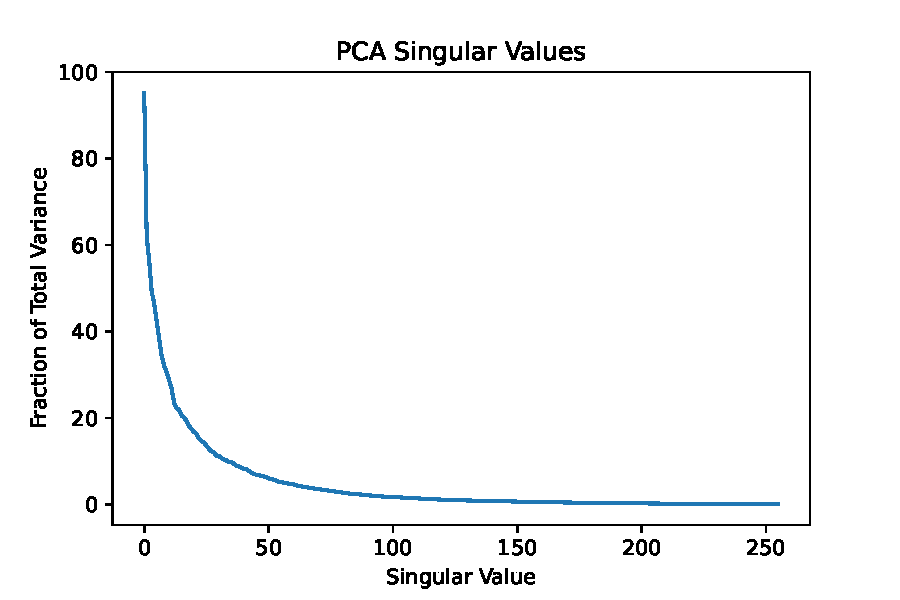
\includegraphics[width=0.4\textwidth]{./PCA Singular Values.pdf}
    \caption{The fraction of the total variance explained by each dimension.}
    \label{fig:singular-values}
\end{figure}

We can see that the first few dimensions are the most important. It looks like after ~150 dimensions, 
the variance is tapered off. This means that the data is not very well represented by the last dimensions. We can 
paint a better picture by looking at the cumulative sum of the variance as well

\begin{figure}[htp]
    \centering
    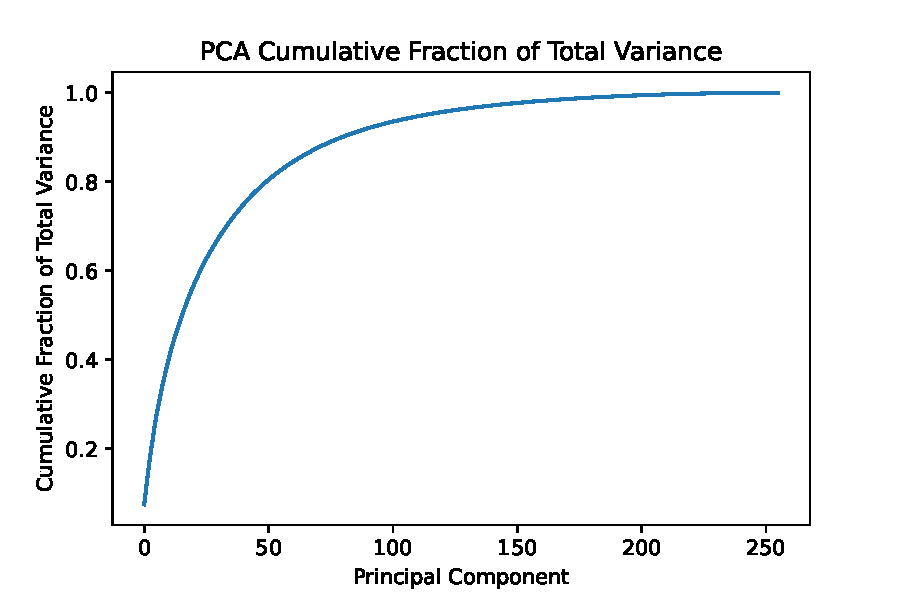
\includegraphics[width=0.4\textwidth]{./PCA Cumulative Fraction of Total Variance.pdf}
    \caption{The cumulative fraction of the total variance explained by each dimension.}
    \label{fig:cumulative-singular-values}
\end{figure}

Our original analysis seems to be correct. We can see that the first few dimensions are the most important 
in terms of their increase. Once we hut 100 principal components, we're above 80 percent of the variance explained.

Looking at the first 16 modes (which according to our graph should be somewhere between 20-40 percent variance), we get the following

\begin{figure}[htp]
    \centering
    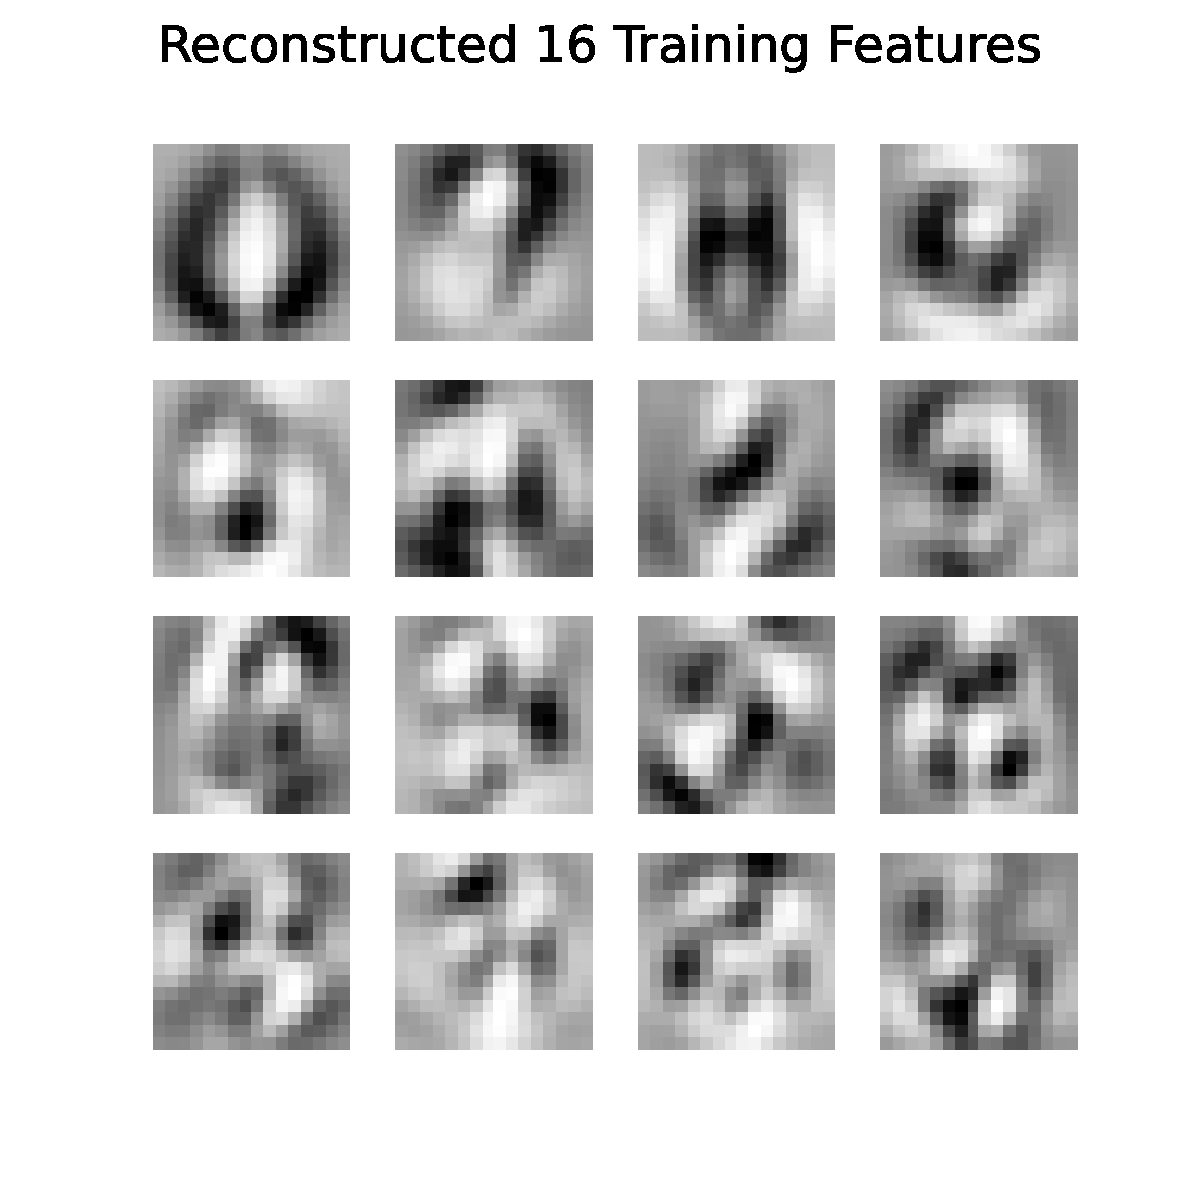
\includegraphics[width=0.4\textwidth]{./Reconstructed 16 Training Features.pdf}
    \caption{The first 16 modes of the training data, applied on 16 sample images.}
    \label{fig:first-16-training-features}
\end{figure}

We can see that these images aren't very decipherable. The third image from the top looks to be 
an 8, but the rest of the images are murky. We should keep in mind that when we reduce dimensionality, 
we lose information. 

Now, we can try to explain the variance according to the Frobenius Norm. I got the following values:
\begin{table}[htp]
    \centering
    \begin{tabular}{|c|c|}
         \hline
         Variance Explained by the Frobenius Norm & Number of Modes Required \\ \hline
         60 percent & 3  \\ \hline
         80 percent & 7  \\ \hline
         90 percent & 14 \\ \hline
    \end{tabular}
    \caption{Variance Explained by the Frobenius Norm and their associated Modes Required.}
    \label{tab:meaningful-label}
\end{table}

We can see that the number of nodes required to explain the variance is increasing with the increase in variance. Surpisingly, we only need 
14 modes to get to 90 percent explained variance. Let's use the first 16 modes to see how accurate of a model we can train. 

When identifying the digits, I got the following results:
\begin{table}[htp]
    \centering
    \begin{tabular}{|c|c|}
         \hline
         Digits & MSE \\ \hline
         1 and 8 Train & 0.0745963381938405 \\ \hline
         1 and 8 Test & 0.08347453537941685  \\ \hline
         3 and 8 Train & 0.18039681693239826  \\ \hline
         3 and 8 Test & 0.2581632921805704  \\ \hline
         2 and 7 Train & 0.09177944633086439  \\ \hline
         2 and 7 Test & 0.13722034799081978  \\ \hline
    \end{tabular}
    \caption{Mean squared error of the model on the training and test data for different pairs of digits}
    \label{tab:mse-table}
\end{table}

We can see that the lowest MSE is for the 1 and 8 pair for both training and test data. 
This means that the model is very accurate. We may think at first that the model is overfitting,
but we can see that the train and test data are very close for the individual pairs. This means that 
we are actually not overfitting, but there is a difference between the pairs. 

One possible explanation may be due to the similarity between the way that digits are written. Recall from 
earlier that when we reduce dimensions, we lose information. This means that some digits may look 
very similar when compared to one another. For instance, 3 and 8 are very similar in the way that they are written. 
This is why they have the highest MSE out of all the pairs. 2 and 7 both have a diagonal line in the middle 
of them, so they are also similar in that fasion. This similarity is not as clear as that between 3 and 8, but the MSE is 
also not as high as that of 3 and 8. 1 and 8 are not very similar, so they have the lowest MSE.


%This is perhaps the most important section of your report. You want to dedicate more space 
% here and present your numerical results in a clear, concise and meaningful way. Also 
% include a discussion of your numerics. Think hard about how you can use 
% your space most efficiently. For example, include subplots and multiple error curves on the 
% same plot etc. Ask us for advice when the time comes. 

% You will most definitely need tables and figures. So here is an example. 

% \begin{table}[htp]
%     \centering
%     \begin{tabular}{| l | c|c | r |}
%          \hline
%          row 1 & column 1  & column 2  \\ \hline
%          row 2 & column 1 & column 2 \\ 
%          row 3 & column 1 & column 2 \\ \hline
%     \end{tabular}
%     \caption{Don't forget to include a caption for your table. Say a few words about what is 
%     being shown.}
%     \label{tab:meaningful-label}
% \end{table}

% Make sure your table is labeled and referenced withing the text using $\backslash$\texttt{ref} as such Table~\ref{tab:meaningful-label}. In fact, you can 
% use $\backslash$\texttt{ref} to cite anything else in the document such as 
% sections (ex. Section~\ref{sec:Introduction}). This will create hyperlinks in your 
% pdf after compilation and automatically update the numbers and tags whenever you change 
% anything. 

% Figures are very similar to tables. Here's an example: 

% % \begin{figure}[htp]
% %     \centering
% %     \includegraphics[width=0.4\textwidth]{./Figs/fig1.pdf}
% %     \caption{Include a descriptive caption for your figure. Also make sure all 
% %     legends, axis labels, and titles are large enough to be readable. You might have 
% %     to reproduce the plots from Python or MATLAB with larger fonts for this purpose. It 
% %     can be annoying the first time you do it but it is crucial.}
% %     \label{fig:meaningful-label}
% % \end{figure}

% You may also need to include multiple figures: 

% % \begin{figure}
% %     \centering
% %     \begin{subfigure}[b]{.3\textwidth}
% %     \includegraphics[width=\textwidth]{./Figs/fig1.pdf}
% %     \caption{First subfigure}
% %     \label{subfig:first}
% %     \end{subfigure}
% %     \begin{subfigure}[b]{.3\textwidth}
% %     \includegraphics[width=\textwidth]{./Figs/fig2.pdf}
% %     \caption{First subfigure}
% %     \label{subfig:second}
% %     \end{subfigure}
% %     \begin{subfigure}[b]{.3\textwidth}
% %     \includegraphics[width=\textwidth]{./Figs/fig3.pdf}
% %     \caption{First subfigure}
% %     \label{subfig:third}
% %     \end{subfigure}
% %     \caption{Caption for entire figure. You don't need to use captions for subfigs so 
% %     feel free to eliminate the subcaption texts to just have the A, B, C labels.}
% %     \label{fig:meaningful-label-2}
% % \end{figure}

% Once again, make sure all your figures are referenced like Figure~\ref{fig:meaningful-label}
% or Figure~\ref{subfig:first} in the text body of the report and discussed 
% in detail. This is where you will make observations about your results and we will 
% look at these very closely. 

% Also note, I am using PDF figures. These give you the best looking graphs but PNG works 
% well too. I advise staying away from JPG as it always looks weird and low quality.]
% Both Python and MATLAB can output figures in PDF or PNG.

\section{Summary and Conclusions}\label{sec:conclusions}
Even with just a simple PCA analysis model with Ridge Regression, we can make a model to 
classify digits to a very high degree of accuracy. Further improvements to the model can 
be to classify all digits at once instead of just pairs, as well as to introduce more 
complicated models such as convolutional neural networks.

% Wrap up your report with a brief summary of what you did and what you discovered. 
% Finish with some conclusions and possibly future directions if any. 

\section*{Acknowledgements}

I am thankful to Professor Hosseini for introducing us to the concept of dimensionality reduction, PCA analysis, and 
different regression models. I am also grateful to the YouTube Channel "StatQuest with Josh Starmer" by Josh Starmer for providing
a visual explanation for the intuition behind PCA dimensionality reduction, and how we can use it to reduce the 
dimensionality of high-dimensional data. 

I am very thankful to my peers taking the class alongside me, they have helped me understand the material as well
as provide a reference to compare my results against. I interacted with them both through Canvas discussion boards
as well as Discord chat. 
% Make sure you you clearly state any help you received including collaborations 
% with your peers. Help from TAs or other mentors, professors, etc that helped you 
% with your assignment. Here's a formal example: 

% The author is thankful to Prof. X for useful discussions about the QR algorithm. 
% We are also thankful to Dr. Strange for suggesting the JAX software package for 
% automatic differentiation. Furthermore, our peer Jean Grey was helpful in 
% implementation of spectral clustering in Python.

\bibliographystyle{abbrv}
\bibliography{HW_References}
\cite{Hunter:2007}
\cite{harris2020array}
\cite{hosseini10_2022}
\cite{hosseini12_2022}
\cite{hosseini13_2022}
\cite{scikit-learn}
 % make sure this matches the .bib file for your corresponding document. You also have to maintain your references in the .bib file 
\end{document}
